\section{Empirical Evidence from Dollar-Pegged Stablecoins}
\label{sec:empirical}

\subsection{Common design and data audit}

We study Kraken USDT/USD, USDC/USD, and DAI/USD transaction bars.  The
primary analysis uses five-minute closes from January 2021 through December
2025; one-minute data provide a separate frequency-consistency exercise.  For
every asset and frequency, the state is $X_t=\log P_t$.  Missing bars are not
imputed, and a transition is used only when both endpoints are observed at
the exact requested horizon.  The main cross-asset sample is the intersection
of exact five-minute transition times across all three assets.  It contains
229,484 pairs and is fixed by a recorded SHA-256 hash before model fitting.

\begin{table}[t]
\centering
\caption{Five-minute data quality and aligned common sample}
\label{tab:three-coin-audit}
\begin{tabular}{lrrrr}
\toprule
Asset & Own-calendar coverage (\%) & Common pairs & Ties (\%) & Min. increment\\
\midrule
USDT & 99.8 & 229,484 & 45.3 & 0.00001 \tabularnewline
USDC & 92.6 & 229,484 & 54.0 & 0.00010 \tabularnewline
DAI & 59.3 & 229,484 & 17.1 & 0.00001 \tabularnewline
\bottomrule
\end{tabular}

\begin{minipage}{0.94\textwidth}
\footnotesize
Notes: Own-calendar coverage is relative to the complete five-minute grid
between the first and last observation in 2021--2025.  Common pairs require
that $t$ and $t+300$ seconds are observed for all three assets.  Ties and
minimum increments are computed on those aligned pairs.  No forward filling
or interpolation is used.
\end{minipage}
\end{table}

Table~\ref{tab:three-coin-audit} shows why the common design is feasible but
also why liquidity cannot be ignored.  USDT has nearly complete own-calendar
coverage, whereas DAI has substantially more missing bars and its coverage
declines late in the sample.  The aligned sample nevertheless exceeds the
pre-specified minimum of 100,000 common exact transitions.  Asset-specific
full histories are retained only as robustness samples; horizontal parameter
comparisons use the aligned calendar.

\begin{figure}[t]
\centering
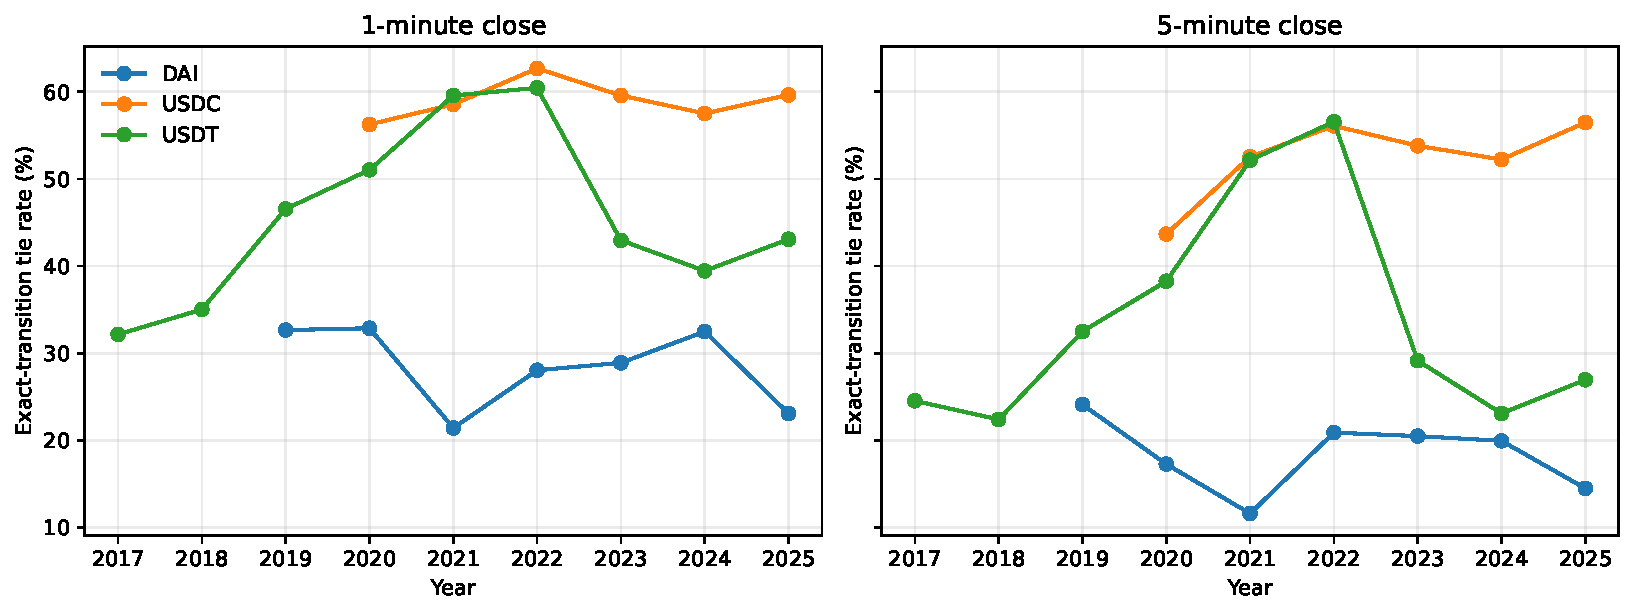
\includegraphics[width=0.88\textwidth]{figures/tie_rate_by_year.pdf}
\caption{Exact-transition tie rates by asset, year, and sampling frequency.}
\label{fig:tie-rate}
\end{figure}

\subsection{Why the continuous point-density likelihood is invalid}

Transaction prices are discrete even when their latent economic value is
modeled continuously.  Figure~\ref{fig:tie-rate} shows pervasive exact ties;
on the aligned five-minute sample their rates are 45.3 percent for USDT,
54.0 percent for USDC, and 17.1 percent for DAI.  The applicable empirical
price increment also changes over time: for example, USDT moves from
$10^{-4}$ in 2021--2022 to $10^{-5}$ from 2023 onward.

This feature invalidates the continuous mixed-OU point-density criterion.
With invariant standard deviation $\tau$, let
\begin{align}
q_h(y\mid x)
&=a_h\phi\!\left(y;
\theta+\rho_h(x-\theta),\tau^2(1-\rho_h^2)\right)
 +(1-a_h)\phi(y;\theta,\tau^2),                 \label{eq:continuous-mou}\\
\rho_h&=e^{-\kappa h},\qquad a_h=e^{-\lambda h}.
\end{align}
For a tied observation $y=x$, as $\kappa\downarrow0$,
\[
 \phi\!\left(x;\theta+\rho_h(x-\theta),
 \tau^2(1-\rho_h^2)\right)
 =\{\tau\sqrt{4\pi\kappa h}\}^{-1}\{1+o(1)\}.
\]
Thus its log contribution diverges as $-\tfrac12\log\kappa$.  For a non-tie,
the OU contribution vanishes, but the reset contribution remains strictly
positive when $\lambda>0$.  Hence the sample log likelihood is unbounded if
there is even one tie.  Finite optimizer output, Hessian diagnostics, and a
continuous-path bootstrap cannot repair this mismatch; the earlier
continuous-density LR calculation is therefore withdrawn.

\subsection{Nearest-tick interval likelihood}

Let $X_i^*$ be a latent log price and let the observed transaction price be
\[
 P_i^{\mathrm{obs}}=\mathcal Q_{\delta_i}(e^{X_i^*}),
\]
where $\delta_i$ is the asset--year tick.  Observing $p_i$ implies
\begin{equation}
 X_i^*\in I_i=
 \left[\log(p_i-\delta_i/2),\log(p_i+\delta_i/2)\right).
 \label{eq:rounding-bin}
\end{equation}
Our present main criterion is the bounded conditional interval approximation
\begin{equation}
 \widetilde q_i(p_i\mid p_{i-1};\psi)
 =\int_{I_i}q_{h_i}\!\left(x\mid\log p_{i-1};\psi\right)\dd x.
 \label{eq:interval-likelihood}
\end{equation}
The Gaussian component probabilities in \eqref{eq:interval-likelihood} are
computed as stable differences of normal CDFs.  Ties now contribute a
probability bounded by one rather than a point density that can diverge.

Equation~\eqref{eq:interval-likelihood} treats the preceding latent state as
the midpoint of its observed bin.  The full structural likelihood instead
recurses
\begin{align}
 \widetilde\alpha_i(x)
 &=\one_{I_i}(x)\int q_{h_i}(x\mid z;\psi)
                 \alpha_{i-1}(z)\dd z,\\
 L_i(\psi)&=\int\widetilde\alpha_i(x)\dd x,
 \qquad \alpha_i(x)=\widetilde\alpha_i(x)/L_i(\psi).       \label{eq:grid-filter}
\end{align}
We implement a deterministic grid version of \eqref{eq:grid-filter} and use it
for finite-sample validation tests.  Sparse/adaptive acceleration is still
required before the full five-year filtered likelihood can replace
\eqref{eq:interval-likelihood}.  Accordingly, all parameter estimates below
are labeled interval-approximation estimates, not final structural MLEs.

Automated tests reproduce the divergence of
\eqref{eq:continuous-mou}, verify that \eqref{eq:interval-likelihood} remains
finite on the same tied sample, test asset-specific and time-varying ticks,
and verify a finite grid-filter likelihood on quantized simulated paths.

\subsection{Full-sample and frozen-training estimates}

We estimate a rounded Gaussian margin first and then fit the OU and mixed-OU
dynamics.  Rates are measured per day.  The full-sample estimates in
Table~\ref{tab:full-interval} are descriptive and use all exact five-minute
pairs available to each asset.  They are not used to score 2024 or 2025.

\begin{table}[t]
\centering
\caption{Full-sample interval-likelihood estimates, 2021--2025}
\label{tab:full-interval}
\begin{tabular}{llrrrrr}
\toprule
Asset & Model & $\theta$ (bp) & $\tau$ (bp) & $\kappa$ & $\lambda$ & Mean half-life (min)\\
\midrule
USDT & OU & 0.671 & 7.359 & 1.608 & 0.000 & 620.7 \tabularnewline
USDT & MOU & 0.671 & 7.359 & 0.705 & 2.773 & 287.0 \tabularnewline
USDC & OU & -1.150 & 18.941 & 1.073 & 0.000 & 930.5 \tabularnewline
USDC & MOU & -1.150 & 18.941 & 0.226 & 0.703 & 1074.7 \tabularnewline
DAI & OU & -0.198 & 21.386 & 4.457 & 0.000 & 223.9 \tabularnewline
DAI & MOU & -0.198 & 21.386 & 0.195 & 27.780 & 35.7 \tabularnewline
\bottomrule
\end{tabular}

\begin{minipage}{0.94\textwidth}
\footnotesize
Notes: Parameters use the asset-specific exact-pair calendar and every
available five-minute pair.  $\theta$ and $\tau$ are latent Gaussian margin
parameters.  The mixed half-life is $\log(2)/(\kappa+\lambda)$ and refers only
to conditional-mean decay.
\end{minipage}
\end{table}

For predictive evaluation, every margin and dynamic parameter is re-estimated
using only 2021--2023 and then frozen.  Table~\ref{tab:training-interval}
reports these estimates separately, eliminating the ambiguity between
full-sample structural description and training-only prediction.

\begin{table}[t]
\centering
\caption{Frozen training interval-likelihood estimates, 2021--2023}
\label{tab:training-interval}
\begin{tabular}{llrrrrr}
\toprule
Asset & Model & $\theta$ (bp) & $\tau$ (bp) & $\kappa$ & $\lambda$ & Mean half-life (min)\\
\midrule
USDT & OU & 1.436 & 8.389 & 1.827 & 0.000 & 546.3 \tabularnewline
USDT & MOU & 1.436 & 8.389 & 0.817 & 2.075 & 345.1 \tabularnewline
USDC & OU & -1.260 & 23.932 & 0.996 & 0.000 & 1002.3 \tabularnewline
USDC & MOU & -1.260 & 23.932 & 0.141 & 1.054 & 835.9 \tabularnewline
DAI & OU & 0.515 & 24.185 & 3.043 & 0.000 & 328.0 \tabularnewline
DAI & MOU & 0.515 & 24.185 & 0.119 & 25.260 & 39.3 \tabularnewline
\bottomrule
\end{tabular}

\end{table}

The two tables also reveal substantial margin instability.  Later years are
narrower for several assets, so matching a full-sample mean and variance is a
calibration identity rather than independent validation of stationarity.
Annual margins, tail probabilities, and out-of-period scores therefore carry
more information than a full-sample mean/scale gate.

\subsection{Aligned cross-stablecoin comparison}

Figure~\ref{fig:cross-drift} estimates local drift nonparametrically on the
aligned sample using equal-frequency state bins.  Most central bins point
toward the zero log peg, but violations remain: 17 of 21 populated USDT bins,
4 of 5 USDC bins, and 23 of 31 DAI bins have the restoring sign.  These are
descriptive curves; synchronized day-block confidence bands remain a gate for
formal local-reversion inference.

\begin{figure}[t]
\centering
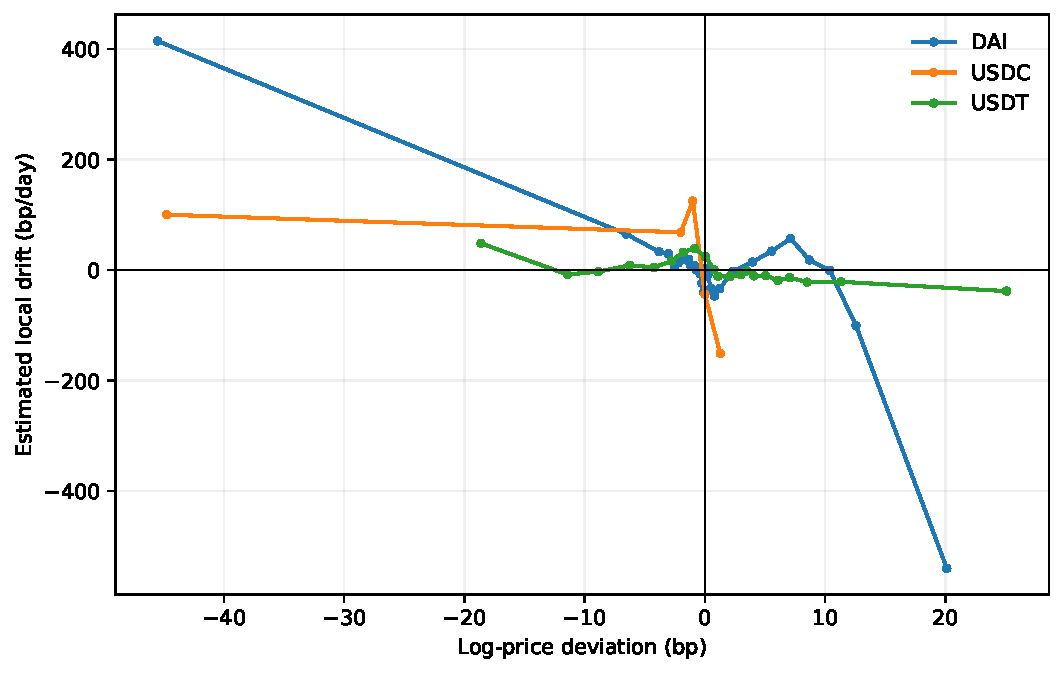
\includegraphics[width=0.82\textwidth]{figures/cross_stablecoin_drift_curves.pdf}
\caption{Nonparametric local drift on aligned exact five-minute pairs.}
\label{fig:cross-drift}
\end{figure}

\begin{table}[t]
\centering
\caption{Mixed-OU interval estimates on the aligned common sample}
\label{tab:cross-parameters}
\begin{tabular}{lrrrrrrr}
\toprule
Asset & $\theta$ (bp) & $\tau$ (bp) & $\kappa$ & $\lambda$ & Base $H$ (h) & Mixed $H$ (h) & $|X|>50$bp (\%)\\
\midrule
USDT & 1.377 & 8.742 & 0.894 & 2.459 & 18.62 & 4.96 & 0.287 \tabularnewline
USDC & -1.350 & 25.209 & 0.130 & 1.235 & 128.22 & 12.19 & 0.257 \tabularnewline
DAI & -0.042 & 23.125 & 0.163 & 28.915 & 102.37 & 0.57 & 0.325 \tabularnewline
\bottomrule
\end{tabular}

\begin{minipage}{0.94\textwidth}
\footnotesize
Notes: The same 229,484 transition times and observation architecture are used
for all assets.  Point differences are not assigned structural significance:
the required synchronous day-block refit and full filtered likelihood have
not passed their gates.
\end{minipage}
\end{table}

Table~\ref{tab:cross-parameters} suggests heterogeneous dependence shapes,
particularly a large DAI refresh estimate.  It does not identify a causal
effect of issuance or collateral design.  All assets share common market
shocks, and DAI has different trading intensity; separate asset bootstraps
would discard that covariance.  Pairwise $\Delta\kappa$ and
$\Delta\lambda$ tests are therefore deliberately left unreported until a
synchronous day-block refit is run on the filtered observation likelihood.

\subsection{Out-of-sample scores with uncertainty}

For each asset and evaluation window, Table~\ref{tab:oos-interval} reports the
paired mean log-observation-probability difference between MOU and OU.  The
standard error clusters all score innovations within a UTC day.  Because both
models assign probability to the same observed tick bin, its width cancels
exactly in the paired comparison.

\begin{table}[t]
\centering
\caption{Frozen-training MOU minus OU interval-score differences}
\label{tab:oos-interval}
\begin{tabular}{llrrrr}
\toprule
Asset & Window & Mean $\Delta$ score & Day-cluster SE & 95\% CI & Pairs\\
\midrule
USDT & Validation 2024 & 0.2737 & 0.0095 & [0.2551, 0.2923] & 105,118 \tabularnewline
USDT & Post-selection 2025 & 0.3167 & 0.0095 & [0.2982, 0.3353] & 104,900 \tabularnewline
USDC & Validation 2024 & 0.5577 & 0.0042 & [0.5495, 0.5658] & 102,499 \tabularnewline
USDC & Post-selection 2025 & 0.6230 & 0.0023 & [0.6185, 0.6275] & 78,698 \tabularnewline
DAI & Validation 2024 & 0.2858 & 0.1026 & [0.0847, 0.4870] & 23,199 \tabularnewline
DAI & Post-selection 2025 & 1.6241 & 0.9640 & [-0.2652, 3.5135] & 13,290 \tabularnewline
\bottomrule
\end{tabular}

\begin{minipage}{0.94\textwidth}
\footnotesize
Notes: All parameters are frozen from 2021--2023.  The 2024 window is
validation; 2025 is post-selection evaluation, not an untouched test sample.
Confidence intervals use UTC-day cluster standard errors.
\end{minipage}
\end{table}

The mixed model improves on OU for USDT and USDC in both windows, with
confidence intervals well above zero.  DAI improves in 2024, but its 2025
interval is wide and includes zero because the late DAI sample is sparse and
episodic.  This is predictive evidence for a non-Gaussian transition mixture;
it does not by itself identify an invariant reset mechanism or a particular
institutional channel.

\subsection{One-to-five-minute semigroup pretest}

A time-homogeneous continuous-time model requires
$P_{5\mathrm m}=(P_{1\mathrm m})^5$ and frequency-invariant daily rates.
We estimate each frequency on 20,000 UTC-day-stratified 2021--2023 pairs with
fixed seeds and recorded index hashes.  This exercise uses the same interval
dynamics but a midpoint-moment margin for computationally transparent pilot
estimation.

\begin{table}[t]
\centering
\caption{Interval-model parameters by sampling frequency}
\label{tab:frequency-parameters}
\begin{tabular}{lrrrrr}
\toprule
Asset & Minutes & $\kappa$ & $\lambda$ & Base $H$ (h) & Mixed $H$ (h)\\
\midrule
USDT & 1 & 2.887 & 3.899 & 5.76 & 2.45 \tabularnewline
USDT & 5 & 0.750 & 2.460 & 22.18 & 5.18 \tabularnewline
USDC & 1 & 0.471 & 3.086 & 35.32 & 4.68 \tabularnewline
USDC & 5 & 0.143 & 1.028 & 116.47 & 14.21 \tabularnewline
DAI & 1 & 0.333 & 122.338 & 50.02 & 0.14 \tabularnewline
DAI & 5 & 0.212 & 23.018 & 78.39 & 0.72 \tabularnewline
\bottomrule
\end{tabular}

\end{table}

\begin{table}[t]
\centering
\caption{Five-minute own fit versus transferred one-minute dynamics}
\label{tab:frequency-transfer}
\begin{tabular}{lrrr}
\toprule
Asset & Five-minute own minus one-minute transfer & Day-cluster SE & 95\% CI\\
\midrule
USDT & 0.1788 & 0.0597 & [0.0619, 0.2957] \tabularnewline
USDC & 0.1854 & 0.0578 & [0.0722, 0.2986] \tabularnewline
DAI & 0.2254 & 0.0249 & [0.1766, 0.2743] \tabularnewline
\bottomrule
\end{tabular}

\begin{minipage}{0.94\textwidth}
\footnotesize
Notes: The one-minute $\kappa$ and $\lambda$ are transferred to the five-minute
kernel while holding the five-minute margin fixed.  Positive values favor the
separately estimated five-minute dynamics.  Confidence intervals cluster by
UTC day.
\end{minipage}
\end{table}

Daily rate estimates differ materially across frequencies, and the
five-minute own dynamics outperform the transferred one-minute rates for all
three assets.  The corresponding 95 percent intervals exclude zero.  This is
a failed semigroup pretest, not a robustness success.  Tick rounding alone,
at least under the midpoint approximation, does not remove high-frequency
microstructure dependence.  Full filtering, richer latent dynamics, or a
two-scale state representation is required before $\kappa$ and $\lambda$ can
be treated as frequency-invariant continuous-time parameters.

\subsection{Theory--evidence consistency and current gates}

The theory predicts that an exact stationary-reset kernel preserves its
chosen invariant margin and multiplies every centered semigroup component by
$e^{-\lambda h}$.  The interval model's positive predictive score differences
are consistent with an additional dependence component.  The cross-frequency
failure, however, prevents a stronger claim that the fitted five-minute rates
are structural continuous-time parameters.  It also reinforces the spectral
identification result in Section~4: second-order decay identifies primarily
$\kappa+\lambda$, while separating the two requires coherent transition shape
across horizons.

The present empirical conclusions therefore pass the bounded-likelihood,
sample-separation, common-calendar, and score-uncertainty gates.  They do not
yet pass the full filtered-likelihood, synchronous cross-asset bootstrap,
multi-horizon identification, or one-to-five-minute semigroup gates.  These
failures are retained as results rather than removed by selecting a more
favorable frequency or asset.
